\chapter{Метод имитации отжига} \label{SimulatedAnnealing}
%\addcontentsline{toc}{chapter}{Имитация отжига}    % Добавляем его в оглавление, если нет нумерации
\noindent
\textit{Имитация отжига} (\emph{simulated annealing}, SA) представляет собой алгоритм решения задачи по поиску глобального оптимума некоторой функции через упорядоченный стохастический поиск, базирующийся на моделировании физического процесса кристализации вещества из жидкого состояние в твердое.

\section{Алгоритм}

\noindent Для описания метода рассмотрим задачу нахождения глобального минимума функции~$F \colon \mathbb{X} \to \mathbb{R}$:
\[
	\mathop{\mathrm{argmin}}_{x \in \mathbb{X}} F(x),
\]

\noindent где~$x = (x_{1},\ldots , x_{m})$~--- вектор всех состояний, $\mathbb{X}$~--- множество всех состояний.

Изначально температура зафиксированна на определенном уровне~$T_0 = const$, $t = 0$.

\begin{enumerate}
	\item  Из множества всех состояний выберем случайный элемент:
	\[
		\widehat{x}_t \equiv x_i,\ i \in (1, ..., m).
	\]

	\item Понизим температуру одним из следующих способов:

		\begin{enumerate}
			\item Больцмановский отжиг
			\begin{equation}
			T_t = \dfrac{T_0}{\ln (1 + t)}, \ t > 0.
			\label{eq:boltzman}
			\end{equation}

			\item Отжиг Коши
			\begin{equation}
			T_t  =  \dfrac{T_0}{t}.
			\end{equation}

			\item Метод тушения
			\begin{equation}
			T_{t + 1} = \alpha T_t,\ \alpha \in (0, 1).
			\label{eq:tushenie}
			\end{equation}

		\end{enumerate}


	\item Пусть следующий элемент зависит от функции из семейства симметричных вероятностных распределений $G \colon \mathbb{X} \to \mathbb{X}$, порождающей новое состояние \cite{Lopatin}:
	\[
	\tilde{x}_t \thicksim G(\widehat{x}_t, T_t).
	\]

	\begin{enumerate}

		\item Часто G выбирается из семейства нормальных распределений:
		\begin{equation}
		\label{eq:normal_G}
		G(\tilde{x}; \widehat{x}, T)
		=
		\dfrac{1}
		{\sqrt{(2\pi)^{D} T}}
		\exp
		\left\lbrace
		\dfrac{- |\tilde{x} - \widehat{x}|^2}{2T}
		\right\rbrace,
		\end{equation}

		где $\widehat{x}$ — математическое ожидание, $T$  — дисперсия, $D$ — размерность пространства всех состояний.

		\item Также для D = 1 используется распределение Коши с плотностью:
		\begin{equation}
		G(\tilde{x}; \widehat{x}, T)
		=
		\dfrac{1}{\pi}
		\dfrac{T}{|\tilde{x}- \widehat{x}|^2 + T^2},
		\end{equation}

		где~$\widehat{x}$~--- параметр сдвига, $T$~--- параметр масштаба.

	\end{enumerate}

	\item Рассчитываем разницу двух функций:
	\[
	\Delta F =
	F(\tilde{x}_t)
	-
	F(\widehat{x}_t).
	\]

	\item Принимаем~$\tilde{x}_t$~или~$\widehat{x}_t$~за новый элемент:
	\[
		\widehat{x}_{t+1}
		=
		\begin{cases}
			\tilde{x}_t,\ \text{с вероятностью}\ \mathbb{P}(\{\widehat{x}_{t+1} = \tilde{x}_t\}) \\
			\widehat{x}_t,\ \text{с вероятностью}\ 1 - \mathbb{P}(\{\widehat{x}_{t+1} = \tilde{x}_t\})
		\end{cases},
	\]

 где вероятность того, что $\widehat{x}_{t+1} \equiv \tilde{x}_t$:

	\begin{equation}
	\mathbb{P}(\{\widehat{x}_{t+1} = \tilde{x}_t\})
	=
	\begin{cases}
	1,
	&
	\Delta F <0
	\\
	\exp
	\left\lbrace
	- \dfrac {\Delta F}{T_t}
	\right\rbrace ,
	&
	\Delta F \geqslant 0
	\end{cases}.
	\end{equation}

	Заметим, чем выше температура, тем больше вероятность принять состояние хуже текущего ($\Delta F \geqslant 0$), --- это позволяет нам не застревать в локальных минимумах. Тем не менее, в течение реализации алгоритма температура начинает постепенно снижаться по законам, расписанным в пункте 2, что в свою очередь понижает вероятность выбрать менее оптимальное решение .

	\item Возвращаемся к пункту 2, пока не выполнен критерий останова.

	Приведем несколько критериев останова:
	\begin{enumerate}.
		\item Ограничить максимально возможное количество итераций алгоритма.
		\item Задать минимальную точность приближения.
		\item Определить минимальное уменьшение функции.
		\item Задать минимально допустимую температуру.
	\end{enumerate}
\end{enumerate}

\end{enumerate}


%%%%%%%%%%%%%%%%%%%%%%%%%%%%%%%%%%%%%%%%%%%%%%%%%%%%%%%%%%%%%%%%%%%%%%%%%%%%%%%%%%%%%%%%%%%%%


\section{Расстановка N ферзей}
\label{section:queens}
\noindent Рассмотрим задачу, в которой необходимо расставить $N$ ферзей на шахматной доске размера $N \times  N$ так, чтобы ни один из них не <<бил>> другого.

В таком случае, множество всех состояний $\mathbb{X}$ будет содержать все возможные расстановки ферзей на шахмотной доске. Общее число возможных расположений $n$ ферзей на $N \times N$-клеточной доске равно:
\[
{\begin{pmatrix} N \times N  \\ n \end{pmatrix}} = \dfrac{N \times N!}{n! (N \times N - n)!}.
\]

Тогда  функция~$F \colon \mathbb{X} \to \mathbb{R}$ будет выдавать количество атак ферзей, и решением данной задачи будет нахождение такого распложения~$x^{*}$, что~$F(x^*) \equiv 0$.

Зафиксируем изначальное расположение ферзей на шахматной доске. Очевидно, что несколько ферзей не могут находиться на одной вертикали или горизонтали, ибо тогда они будут находиться под ударом друг-друга. Следовательно, наша задача сужается к поиску расположения:
\begin{equation}
x* = (q_1, ..., q_n) = \{(1, h_1), ..., (n, h_n)\}, h_1 \neq ...  \neq h_n,
\end{equation}

где $(i, h_i)$ — расположение ферзя $q_i$ на i-ой вертикали по горизонтали $h_i$.

Отметим, что такая задача имеет $N!$ решений.

\newgame
\fenboard{q7/1q6/2q5/3q4/4q3/5q2/6q1/7q w - - 0 1}

\begin{figure}[h!]
	\begin{center}
		\showboard
		\legend{}
		\caption{ --- Изначальное расположение.}
		\label{img:nonopt}
	\end{center}
\end{figure}
Определим функцию, которая будет создавать изначальное неоптимальное расположение, в общем виде. Учитем, что несколько ферзей не могут находиться на одной вертикали или горизонтали.

\begin{pyin}
def queens(N):
  ver = np.arange(1, N + 1)
  hor = np.arange(1, N + 1)
  np.random.shuffle(hor)
  return np.column_stack((ver, hor)) # получаем массив
  # размерности (N, 2), отождествляющий расположение ферзей
\end{pyin}

Выведем первоначальное расположение ферзей для стандартной доски $8 \times 8$, где первый столбец массива — расположение по вертикали, второй столбец массива — расположение по горизонтали. Для наглядности — презентации оптимизационного процесса — выстроим изначальную расстановку на главной диагонали (рис. \ref{img:nonopt}).


\begin{pyin}
matrix = queens(8)
matrix
\end{pyin}

\begin{pyout}
array([[1, 1],
       [2, 2],
       [3, 3],
       [4, 4],
       [5, 5],
       [6, 6],
       [7, 7],
       [8, 8]])
\end{pyout}


Функция $F$, которая выявляет количество атак ферзей, выглядит следующим образом:
\begin{pyin}
def F(Q, N):
  cnt = 0
  for i in range(N):
     for j in range(i + 1, N):
         if abs(Q[i, 0] - Q[j, 0]) == abs(Q[i, 1] - Q[j, 1]):
             cnt += 1
  return cnt * 2 # учитываем взаимные атаки
\end{pyin}

Посмотрим, сколько атак у исходной расстановки.
\begin{pyin}
F(matrix, 8)
\end{pyin}

\begin{pyout}
56
\end{pyout}

В нашей задаче функция $G$ будет случайной незначительной перестановкой номеров горизонтали в исходном наборе:

\begin{pyin}
def G(Q, N):
  pos = Q.copy()
  while True:
     i = np.random.randint(0, N - 1)
     j = np.random.randint(0, N - 1)
     if i != j:
        break
  pos[i, 1], pos[j, 1] = pos[j, 1], pos[i, 1]
  return pos # получаем новое расположение
\end{pyin}

Теперь выведем и сам метод имитации отжига, используя метод тушения для понижения температуры (\ref{eq:tushenie}).

\begin{pyin}
def SA(Q, T, schedule):
  N = np.shape(Q)[0]
  x_hat = Q.copy()
\end{pyin}

\begin{pyprint}
  while F(x_hat, N) != 0:
     x_tilda = G(x_hat, N)
     delta = F(x_tilda, N) - F(x_hat, N)
     prob = np.exp(- delta / T)
     if (delta < 0) or (prob >= np.random.random()):
        x_hat = x_tilda
     # используем метод тушения для понижения температуры
     T *= schedule
  return x_hat
\end{pyprint}


\newgame
\fenboard{2q5/4q3/1q6/7q/q7/6q1/3q4/5q2 w - - 0 1}

\begin{figure}[h!]
	\begin{center}
		\showboard
		\legend{}
		\caption[р]{ --- Оптимальное расположение}
		\label{img:opt}
	\end{center}
\end{figure}
Так для нашего примера с гиперпараметрами $T_0 = 100, \alpha = 0.9$ мы получаем следующее оптимальное решение:

\begin{pyin}
SA(matrix, 100, 0.9)
\end{pyin}

\begin{pyout}
array([[1, 4],
       [2, 6],
       [3, 8],
       [4, 2],
       [5, 7],
       [6, 1],
       [7, 3],
       [8, 5]])
\end{pyout}

\begin{figure}[h!]
\centering
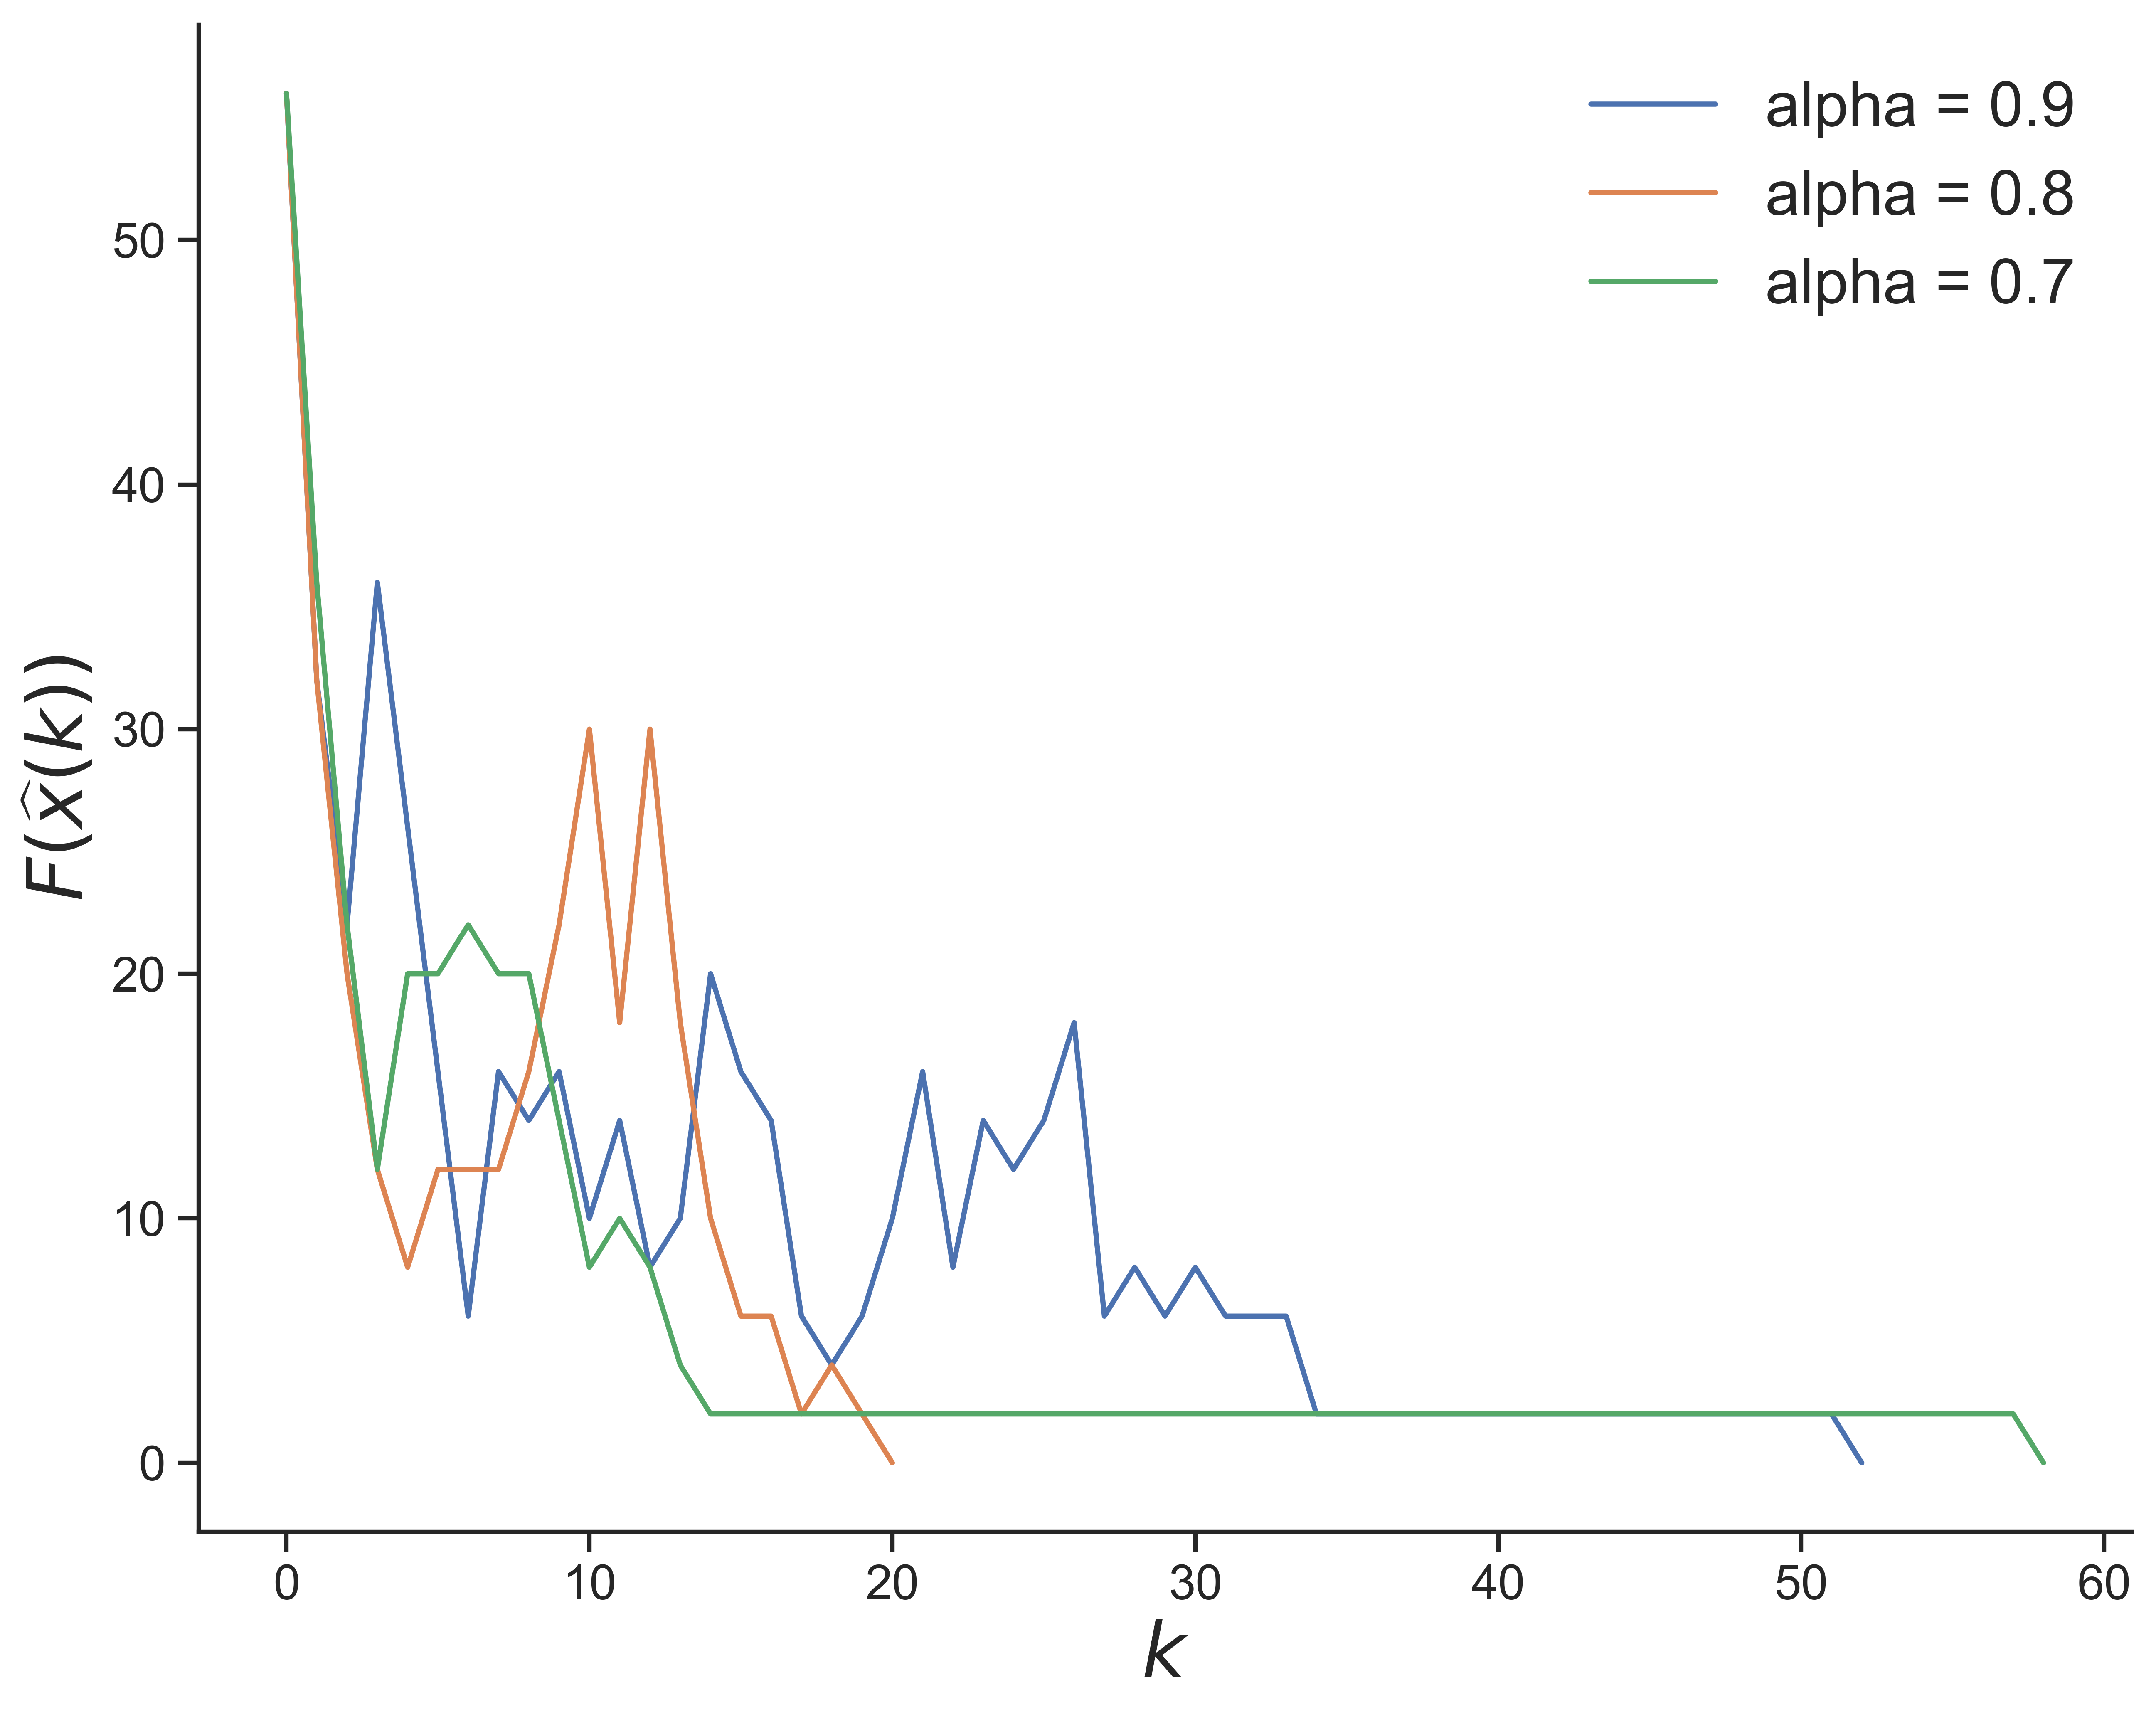
\includegraphics [width=110mm]{queens8}
\caption{ --- Оптимизация расстановки 8 ферзей  в зависимости от гиперпараметра $\alpha$.}
\label{img:queens8}
\end{figure}

\begin{figure}[h!]
\centering
\includegraphics [width=110mm]{queens25}
\caption{ --- Оптимизация расстановки 50 ферзей  в зависимости от гиперпараметра $\alpha$.}
\label{img:queens25}
\end{figure}

Можно заметить, что именно для этой задачи,чем меньше гиперпараметр $\alpha$, тем меньше требуется итераций для нахождения оптимального решения (рис. \ref{img:opt}). Обычно, напротив, $\alpha$ должна быть как можно ближе к 1 \ref{Shamin1}, чтобы позволить алгоритму найти другие, возможно, более оптимальные решение. Также стоит отметить достаточно большой недостаток алгоритма имитации отжига: решение не всегда может <<сойтись>>. Тогда необходимо повторно запускать данный метод. Нашу задачу можно усложнить и, к примеру, сформировать оптимальную расстановку для 50 или более ферзей (рис. \ref{img:queens25}), которую она также достаточно эффективно решает.



%%%%%%%%%%%%%%%%%%%%%%%%%%%%%%%%%%%%%%%%%%%%%%%%%%%%%%%%%%%%%%%%%%%%%%%%%%%%%%%%%%%%%%%%%%%%%


\section{Минимизация негладкой функции}

\noindent Воспользуемся алгоритмом имитации отжига для нахождения глобального минимума следующей функции:
\[
f(x) = x^2 (1 + |\sin 80x|).
\]

	\begin{figure}[h]
	\centering
	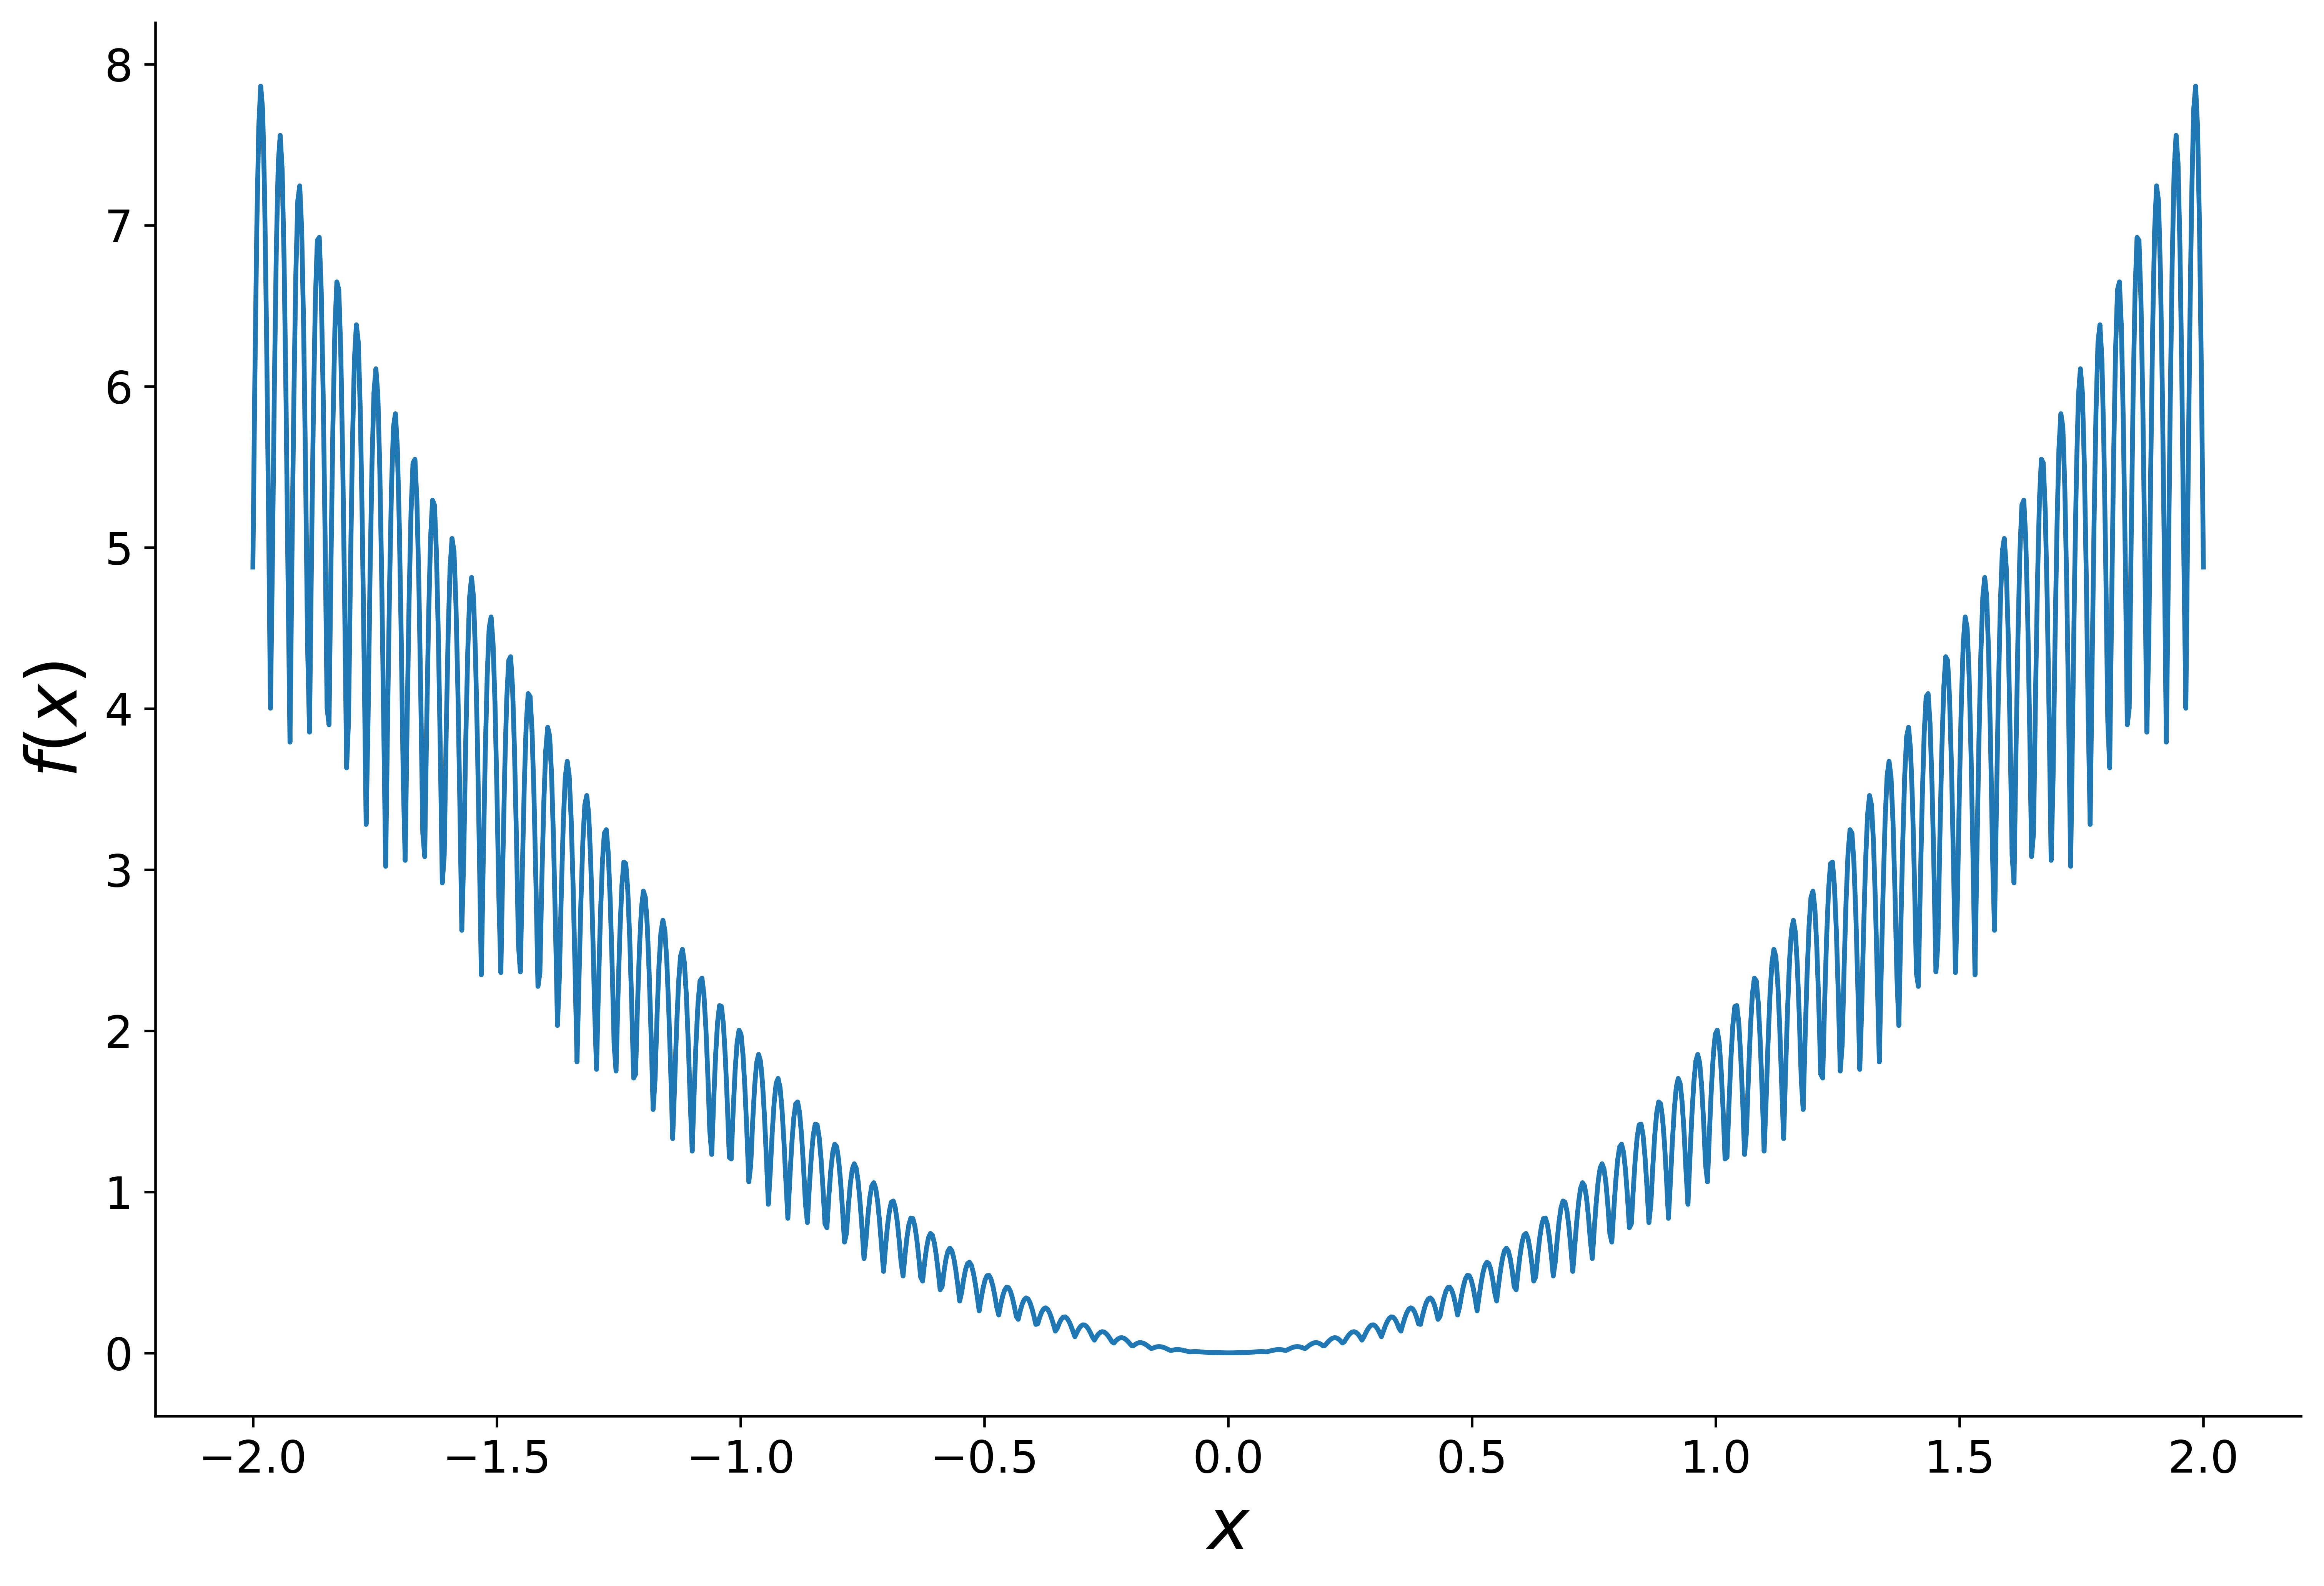
\includegraphics[width=110mm]{func_min}
	\caption{}
	\label{img:func_min}
\end{figure}

Стандартные методы оптимизации --- к примеру, метод градиентного спуска, --- в данном случае не применимы. Заданная функция не дифференцируема. Также она имеет очень большое количество локальных экстремумов, что затрудняет, к примеру, мультистарт --- запуск градиентного спуска из разных начальных направлений.

Применим наш алгоритм к данной задачи. Пусть~$T_0 = 0.6$. Для понижения температуры будем использовать Больцмановский отжиг~(\ref{eq:boltzman}), а в качестве функции вероятностных распределений $G$ будем использовать семейство нормальных распределений~(\ref{eq:normal_G}).

\begin{pyin}
def SA(space, T, epsilon): # за space берется np.linspace(-2,2,1000)
  x_hat = np.random.choice(space)
  T_0 = T
  t = 1
\end{pyin}

\begin{pyprint}
	while True:
		 x_tilda = np.random.normal(x_hat, T)
		 delta = F(x_tilda) - F(x_hat)
		 prob = np.exp(- delta / T)
     if (delta < 0) or (prob >= np.random.random()):
        x_hat = x_tilda
     if (x_hat < epsilon) and (x_hat > 0):
        return x_hat
     T = T_0 / np.log(1 + k)
     t += 1
\end{pyprint}

Остановка итерационного процесса и скорость метода зависят от того, насколько близко мы хотим приблизиться к глобальному минимуму. Так, при точности~$1e-1}$ --- что является достаточно большой погрешностью, --- для 1000 итераций алгоритма метод отжига находит глобальный минимум в среднем за~1.97e-3~секунды со стандартным отклонением в~3.47e-5~секунды. Однако, увеличив точность до~$1e-6$, среднюю скорость занимает уже~1.27~секунды со стандартным отклонением в~2.1e-5~секунды (рис. \ref{img:func_min1}).

\begin{figure}[h!]
	\centering
	\includegraphics[width=150mm]{func_min1}
	\caption{ --- Оптимизационный процесс в зависимости от точности.}
	\label{img:func_min1}
\end{figure}

\newpage

\section{Задача коммивояжера}
\label{section:TSP}

\noindent \emph{Задача коммивояжера} (\emph{traveling salesman problem}, TSP) является образцовым методом проверки многих оптимизационных алгоритмов и заключается в поиске кратчайшего маршрута между городами. Путь должен быть проложен так, чтобы маршрут единственно проходил через все города и его конечная точка совпадала с  изначальной.

TSP имеет множество приложений в планировании и логистике, а также выступает в качестве подзадачи во многих других областях.  В таком случае города могут представлять, к примеру, клиентов, а расстояние между городами — время или стоимость путешествия.

\begin{figure}[h!]
\centering
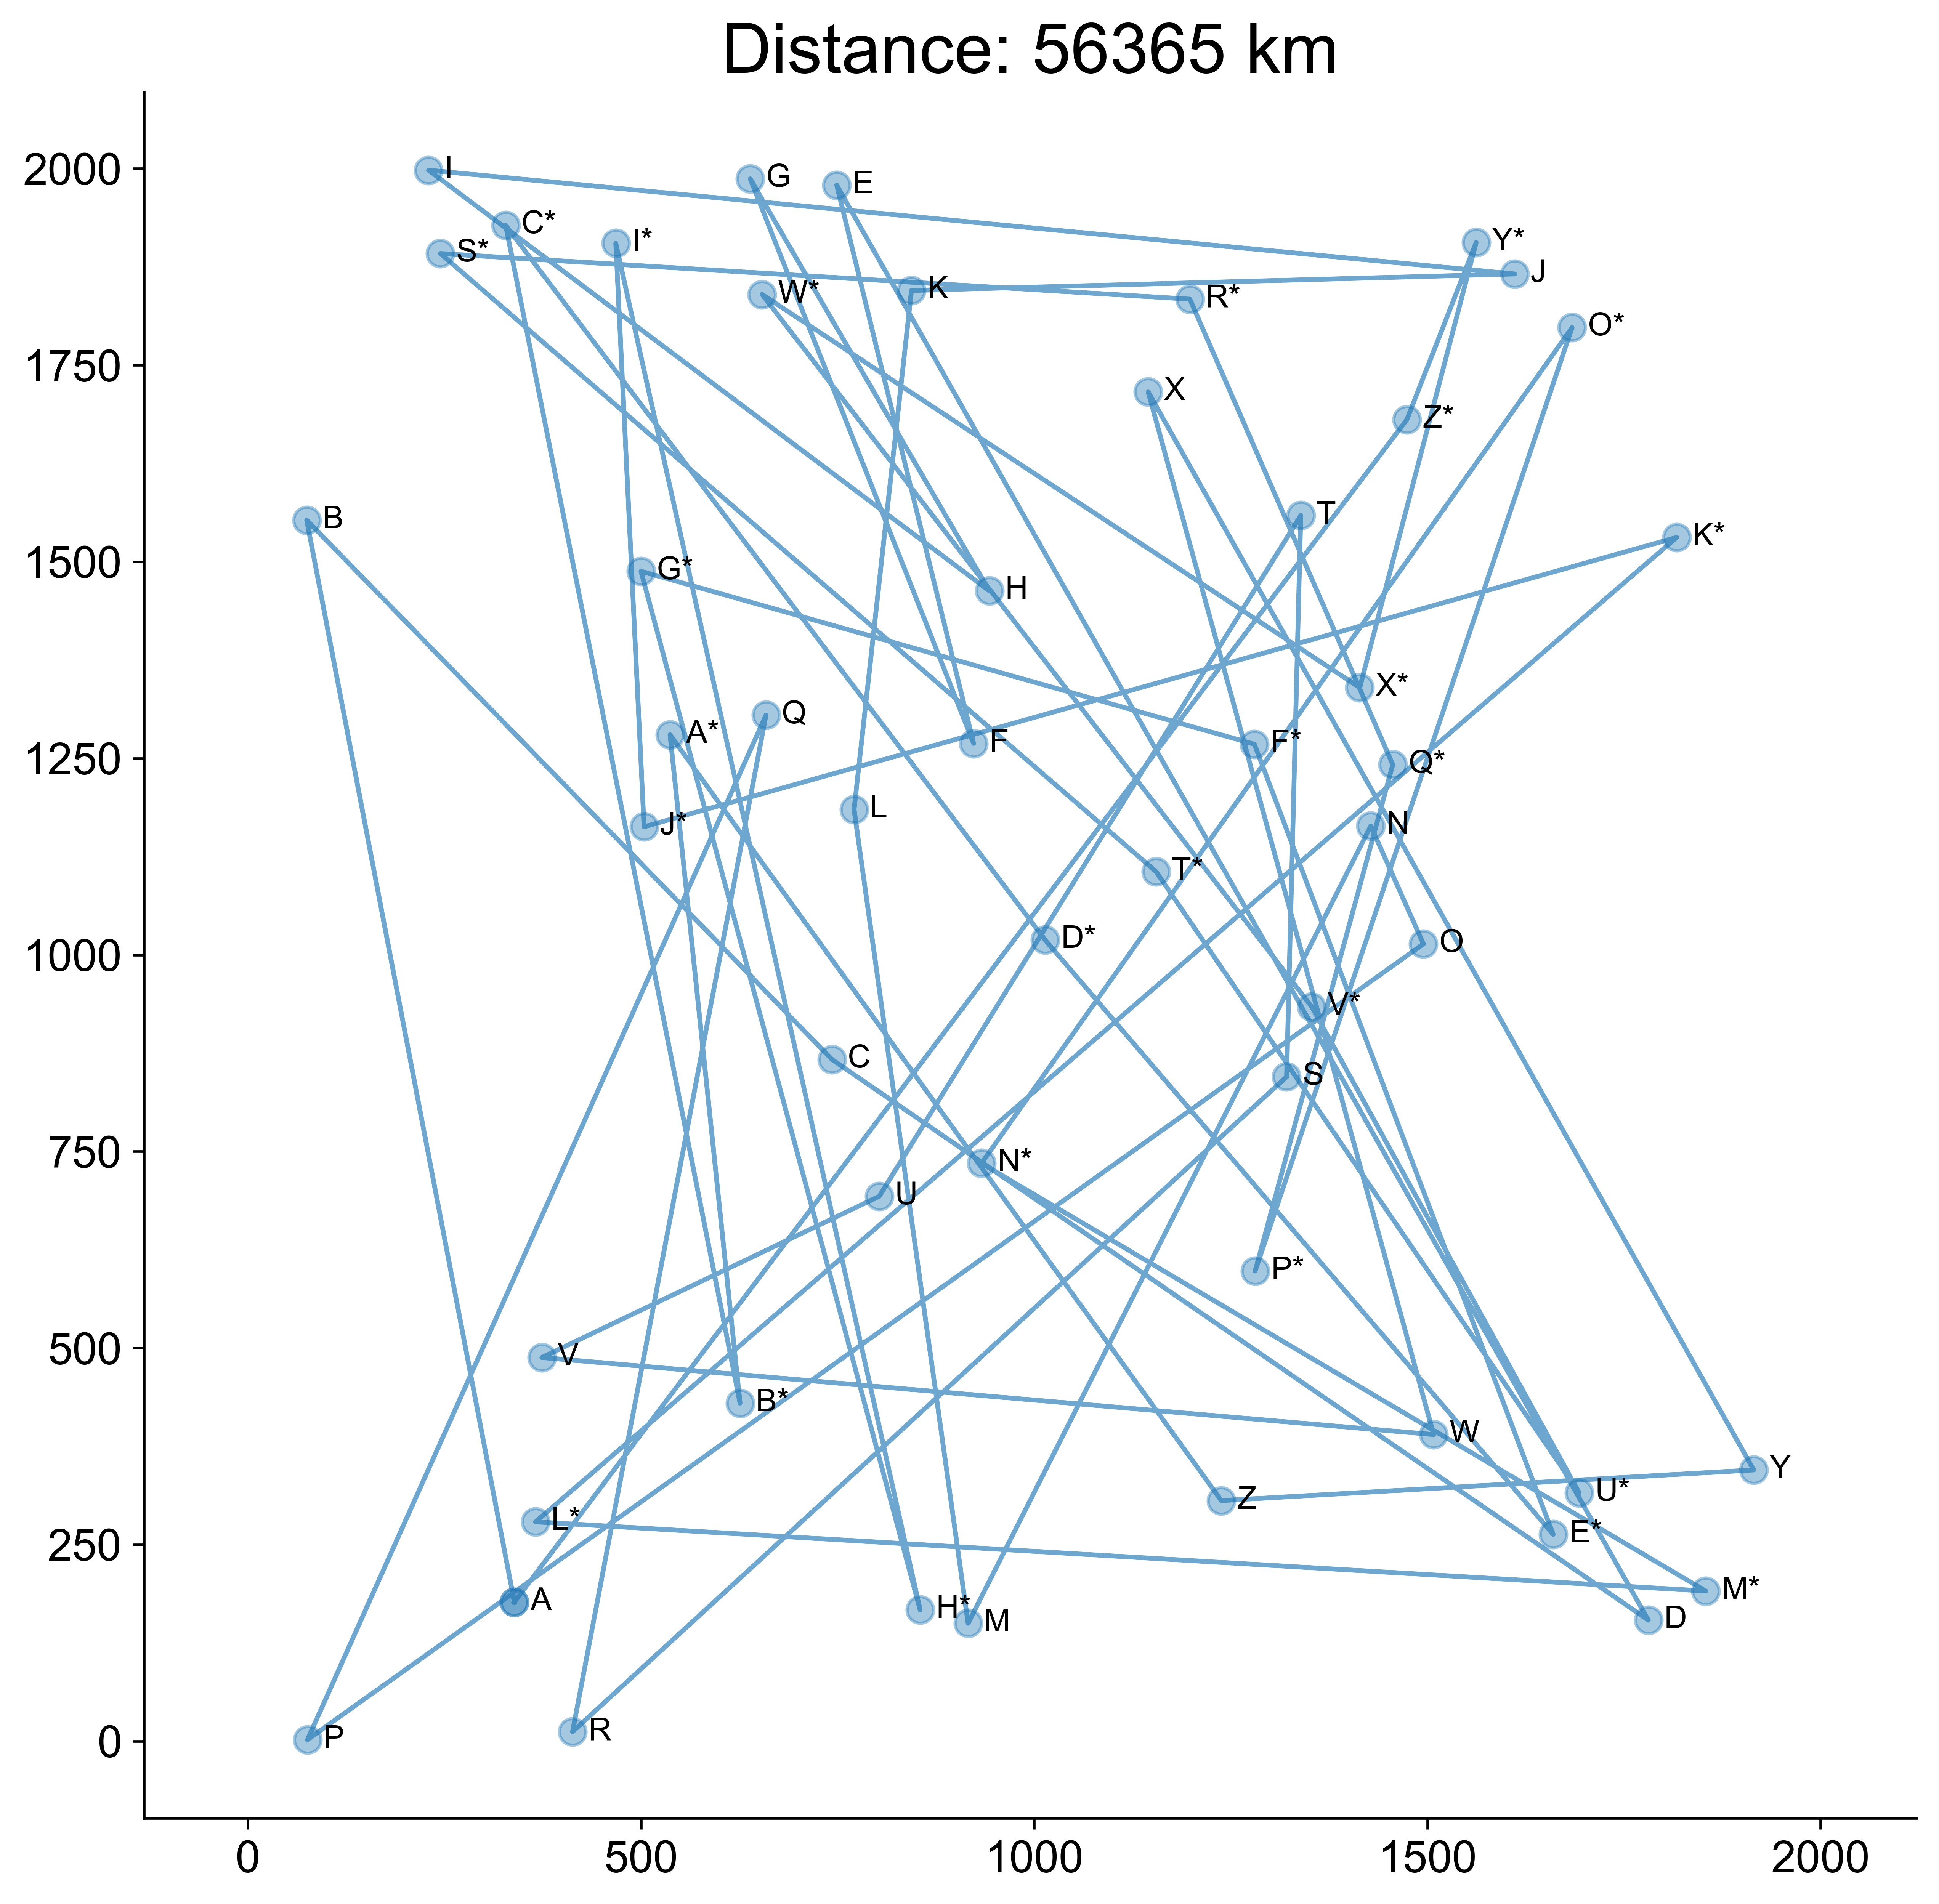
\includegraphics [width=110mm]{TSP1}
\caption{ --- Изначальный маршрут для 26-ти городов.}
\label{img:tsp1}
\end{figure}

Для нашего примера создадим карту. Функция \texttt{map\_city} будет принимать желаемое количество городов в качестве входных данных и выдавать два списка, из которых далее создается общий список кортежей. Первым элементом кортежа является наименование города, а вторым --- его расположение в декартовой системе координат.

\begin{pyin}
def map_city(cities_num):
  letters = [chr(i) for i in range(65, 65 + cities_num)]
  coord = np.random.randint(1, 500, size=(cities_num, 2))
\end{pyin}

\begin{pyprint}
  return letters, coord
\end{pyprint}
Наш маршрут будет состоять из 26-ти городов.

\begin{pyin}
names, cities = map_city(26)
store_val = list(zip(names, cities))
\end{pyin}


Определим расстояние от города i до всех остальных посредством функции \texttt{distance\_dict}. Для измерения расстояния между городами будем использовать евклидову метрику. Напомним, что евклидово расстояние между точками~$x = (x_1, ..., x_d)$~и~$u = (u_1, ..., u_d)$~задается как
\[
\rho (x, u)
=
\sqrt{
\sum_{i = 1}^d \limits
(x_i - u_i)^2
}.
\]

\begin{pyin}
def distance_dict(cities, n):
  d = dict()
  for i in range(n):
     city = dict()
     for j in range(n):
        if i == j:
           continue
        c_a = cities[i][1]
        c_b = cities[j][1]
        dist = np.sqrt((c_a[0] - c_b[0])**2 + (c_a[1] - c_b[1])**2)
        city[cities[j][0]] = dist
     d[cities[i][0]] = city
  return d
\end{pyin}


\begin{pyin}
cities_d = distance_dict(store_val, len(store_val))
\end{pyin}


Функция $F$ для подсчета общего расстояния путешествия:

\begin{pyin}
def F(path, cities):
  dist = 0
  for i in range(len(path) - 1):
     dist += cities[path[i]][path[i + 1]]
  dist += cities[path[i + 1]][path[0]]
  return dist
\end{pyin}

За функцию $G$ будет выступать простая перестановка как и в задаче о расположении $N$ ферзей (разд. \ref{section:queens}).

\begin{pyin}
def G(path, n):
  pos = path.copy()
  while True:
     i = np.random.randint(0, n - 1)
     j = np.random.randint(0, n - 1)
     if i != j:
        break
     pos[i], pos[j] = pos[j], pos[i]
  return pos
\end{pyin}

\begin{figure}[h!]
\centering
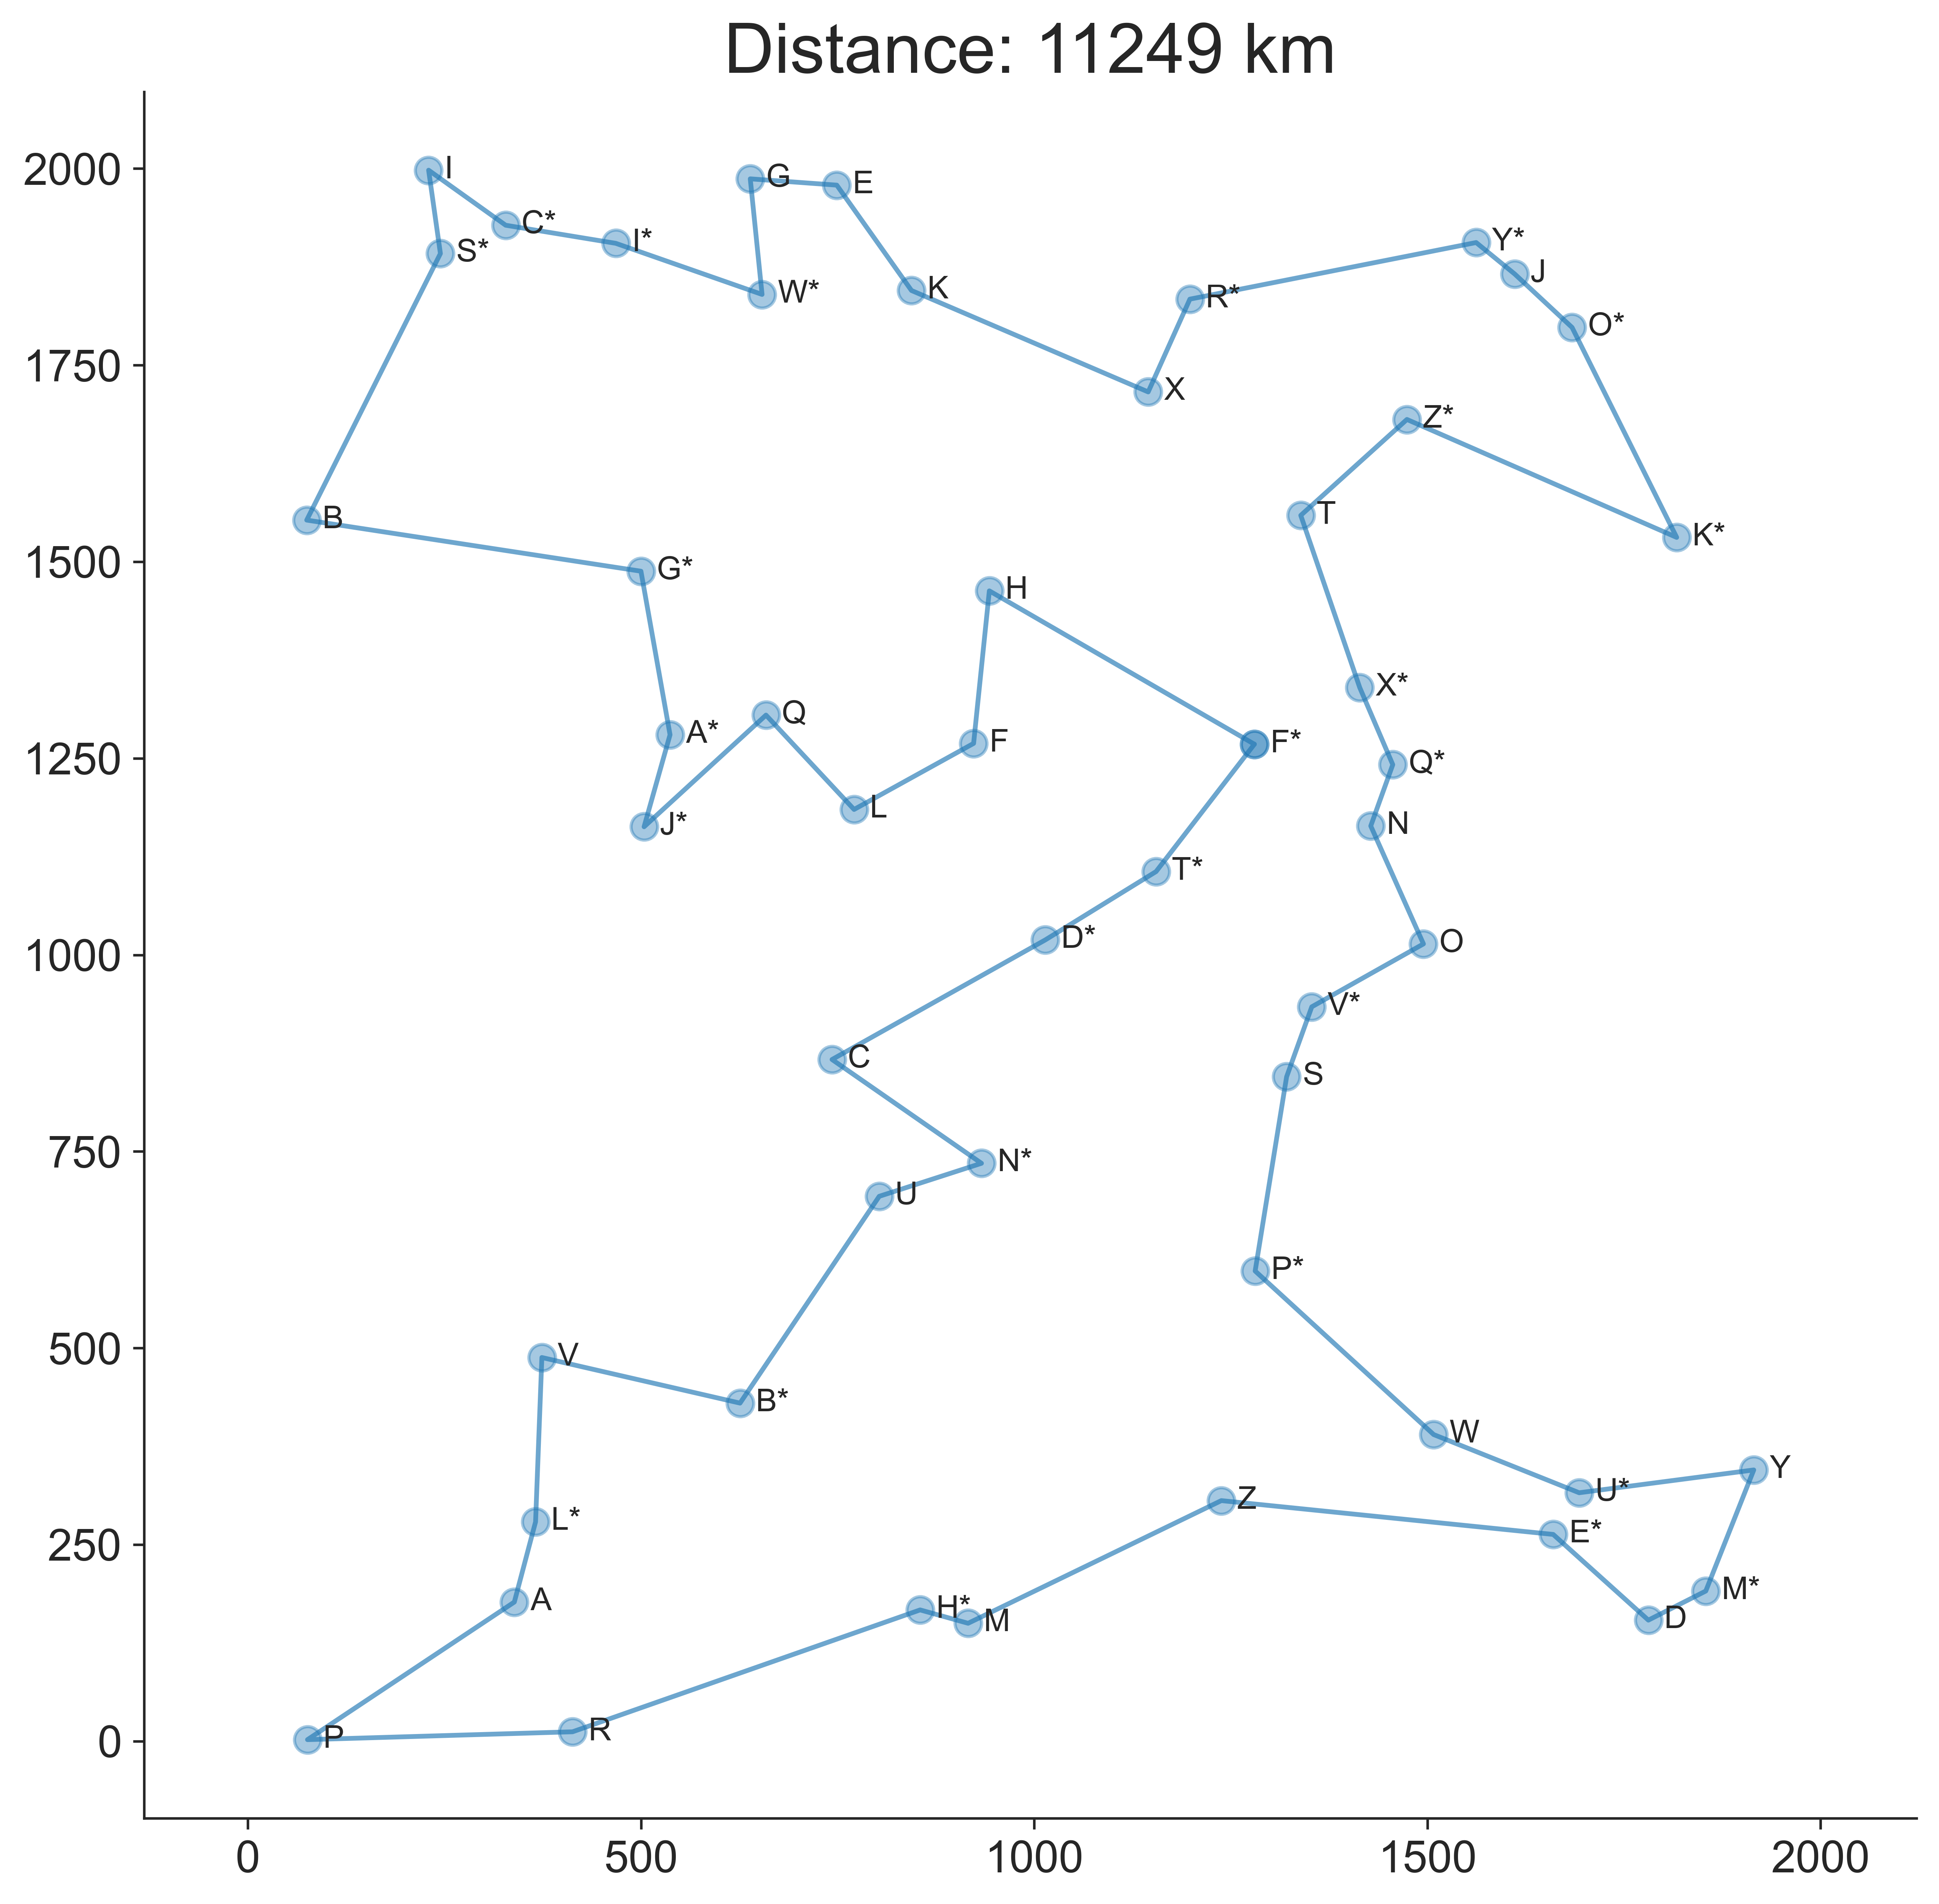
\includegraphics [width=110mm]{TSP2}
\caption{ --- Применение метода отжига для построения оптимального маршрута для 26-ти городов.}
\label{img:tsp2}
\end{figure}


Для понижения температуры используем Больцмановский отжиг~(\ref{eq:boltzman}).

\begin{pyin}
def SA(path, T):
  path_hat = path
  n = len(path_hat)
  np.random.shuffle(path_hat)
  T_0 = T
  k = 1
  for i in range(100000):
     path_tilda = G(path_hat, n)
     delta = F(path_tilda, cities_d) - F(path_hat, cities_d)
     prob = np.exp(- delta / T)
\end{pyin}

Теперь построим оптимальный маршрут (рис.~\ref{img:tsp2}).

\begin{pyin}
path_opt = SA(names, 100)
\end{pyin}

Несмотря на то, что метод отжига сократил преодалеваемую дистанцию, TSP была решена неидеально. К примеру, можно выделить соединение вершин E-S-L-V: очевидно, что оно не оптимально, поскольку путь E-L-S-V имеет меньшее расстояние. Тем не менее, сам маршрут весьма удовлетворителен.

\section{Вывод}

\noindent
Рассмотрев алгоритм имитации отжига, выявим его плюсы и минусы.
\noindent
\begin{table}[h!]
	\caption{Метод отжига}
	\label{table:SA}
	\begin{tabular}{
	  p{\dimexpr.5\linewidth-2\tabcolsep-1.3333\arrayrulewidth}% column 1
	  p{\dimexpr.5\linewidth-2\tabcolsep-1.3333\arrayrulewidth}% column 2
	  }
	  \toprule
	  \centering Преимущества & \centering\arraybackslash Недостатки \\
		\midrule
	  1.~Не требует дифференцируемости и непрерывности исследуемой функции & 1.~Не подходит для задач с небольшим количеством локальных экстремумов  \\[.5\normalbaselineskip]
		2.~Используется для широкого класса задач & 2.~Не всегда сходится к решению \\[.5\normalbaselineskip]
	  3.~Не застревает в локальных экстремумах &  3.~Для сложных задач дает вполне приемлемое, однако не оптимальное, решение \\[.5\normalbaselineskip]
		4.~Имеет простую реализацию &  \\[.5\normalbaselineskip]
		\bottomrule
	\end{tabular}
\end{table}
